% EnergyMind Tunisia - TSYP14 Phase 1 report (Overleaf project, compile with pdfLaTeX)
\documentclass[10pt,a4paper]{article}

\usepackage[T1]{fontenc}
\usepackage[utf8]{inputenc}
\usepackage{mathptmx}
\usepackage[scaled=.92]{helvet}
\usepackage{courier}
\usepackage[a4paper,top=2.4cm,bottom=2.3cm,left=2.2cm,right=2.2cm]{geometry}
\usepackage{microtype}
\usepackage{titlesec}
\usepackage{enumitem}
\usepackage{booktabs,tabularx,array,multirow}
\usepackage[table]{xcolor}
\usepackage{graphicx}
\usepackage{caption}
\usepackage{fancyhdr}
\usepackage{needspace}
\usepackage{tocloft}
\setlength{\cftbeforesecskip}{4pt}\setlength{\cftbeforesubsecskip}{0pt}\renewcommand{\cfttoctitlefont}{\sffamily\Large\bfseries}\renewcommand{\cftaftertoctitle}{\vspace{-0.1em}}\renewcommand{\cftsecfont}{\sffamily\bfseries}\renewcommand{\cftsubsecfont}{\small}\renewcommand{\cftsubsecpagefont}{\small}
\usepackage{amsmath,amssymb}
\usepackage{tikz,pgfplots}
\usepackage[hyphens]{url}
\usepackage[hidelinks,pdfusetitle]{hyperref}
\pgfplotsset{compat=1.16}
\usetikzlibrary{arrows.meta,positioning,fit,calc,patterns,backgrounds}

\hypersetup{pdftitle={EnergyMind Tunisia - Phase 1 Report},pdfauthor={}}
\urlstyle{tt}
\makeatletter\g@addto@macro\UrlBreaks{\do\-\do\_\do\=\do\&\do\?}\makeatother
\Urlmuskip=0mu plus 2mu\relax

% ---------- layout
\setlength{\parindent}{0pt}
\setlength{\parskip}{4.6pt plus 1pt}
\renewcommand{\arraystretch}{1.15}
\setlist{nosep,leftmargin=1.2em,itemsep=2pt}
\raggedbottom
\setcounter{tocdepth}{2}
\renewcommand{\topfraction}{0.9}\renewcommand{\bottomfraction}{0.8}
\renewcommand{\textfraction}{0.1}\renewcommand{\floatpagefraction}{0.8}
\setlength{\textfloatsep}{12pt plus 2pt minus 4pt}\setlength{\intextsep}{10pt plus 2pt minus 2pt}

\titleformat{\section}{\sffamily\Large\bfseries}{\thesection}{0.7em}{}[\vspace{-0.1em}\rule{\textwidth}{1.1pt}]
\titlespacing*{\section}{0pt}{18pt}{9pt}
\titleformat{\subsection}{\sffamily\large\bfseries}{\thesubsection}{0.6em}{}
\titlespacing*{\subsection}{0pt}{11pt}{4pt}
\titleformat{\subsubsection}{\sffamily\normalsize\bfseries}{}{0em}{}
\titlespacing*{\subsubsection}{0pt}{7pt}{3pt}

\captionsetup{font={small,sf},labelfont=bf,labelsep=period,skip=5pt}
\captionsetup[table]{position=top,skip=4pt}

\pagestyle{fancy}
\fancyhf{}
\renewcommand{\headrulewidth}{0.4pt}
\fancyhead[L]{\sffamily\scriptsize EnergyMind Tunisia \,$\cdot$\, Phase 1 Report}
\fancyhead[R]{\sffamily\scriptsize TSYP14 Technical Challenge}
\fancyfoot[L]{\sffamily\scriptsize github.com/azert88/energymind-tunisia}
\fancyfoot[R]{\sffamily\scriptsize\thepage}

\let\oldsection\section
\renewcommand{\section}{\needspace{9\baselineskip}\oldsection}
\let\oldsubsection\subsection
\renewcommand{\subsection}{\needspace{6\baselineskip}\oldsubsection}

% ---------- macros
\newcommand{\code}[1]{\texttt{\small\detokenize{#1}}}
\newcommand{\hdr}{\rowcolor{black!12}}
\newcommand{\goalbadge}[1]{{\sffamily\scriptsize\bfseries\fbox{\,#1\,}}}
\newcolumntype{Y}{>{\raggedright\arraybackslash}X}
\newcolumntype{C}{>{\centering\arraybackslash}X}
\newcommand{\HFURL}{https://www.kaggle.com/datasets/azertyqsdfghqsdfgh/pes-test}

\tikzset{
  box/.style={draw=black,rounded corners=2pt,align=center,font=\sffamily\scriptsize,inner sep=3pt,fill=white,thick,minimum height=8mm},
  gbox/.style={box,fill=black!9},
  hbox/.style={box,fill=black!20,line width=1.1pt},
  dbox/.style={box,dashed},
  arr/.style={-{Latex[length=1.8mm]},thick},
  darr/.style={-{Latex[length=1.8mm]},thick,dashed},
  barr/.style={{Latex[length=1.8mm]}-{Latex[length=1.8mm]},thick},
  tag/.style={font=\sffamily\bfseries\fontsize{6.5}{7.5}\selectfont,text=black!70}
}

\begin{document}

% =============================================================== COVER
\begin{titlepage}
\thispagestyle{empty}
\vspace*{-0.2cm}
{\sffamily\scriptsize IEEE TSYP14 \,$\cdot$\, TECHNICAL CHALLENGE \,$\cdot$\, ENERGYMIND TUNISIA}\\[-4pt]
\rule{\textwidth}{2.2pt}
\vspace{4.6cm}

{\sffamily\fontsize{46}{50}\selectfont\bfseries EnergyMind\\[4pt] Tunisia}\\[16pt]
{\itshape\Large A trust layer between raw meter data\\ and automated action}\\[12pt]
\rule{4.5cm}{0.9pt}\\[16pt]
{\sffamily\Large\bfseries Phase 1 Report}\\[4pt]
{\sffamily\large Project proposal: scope, objectives, data and anomaly-simulation plan, preliminary design for each of the four challenge goals}

\vspace{1.4cm}
{\itshape\small Detect with numerical evidence.\\ Explain with inspectable sources.\\ Act through explicit authority.\\ Learn only from reviewed outcomes.}

\vfill
{\sffamily\scriptsize\bfseries DATASET (KAGGLE)}\\[1pt]
{\ttfamily\scriptsize \url{\HFURL}}\\[6pt]
{\sffamily\scriptsize\bfseries CODE (GITHUB)}\\[1pt]
{\ttfamily\footnotesize \url{https://github.com/azert88/energymind-tunisia}}\\[8pt]
\rule{\textwidth}{0.8pt}\\[-2pt]
{\sffamily\scriptsize Submitted 15 October 2026}\\[1pt]
{\sffamily\scriptsize\itshape Challenge: Architects of the Energy Noosphere: A Human-AI Collective Intelligence Network for Energy Resilience}
\end{titlepage}

% =============================================================== SUMMARY
\section*{Summary}
\addcontentsline{toc}{section}{Summary}
Tunisia's electricity system now fails at the peak: in July 2026 demand reached a record 4,924~MW and STEG resorted to rotating load shedding. Meanwhile rooftop solar and smart meters keep spreading, and every new device is a new source of numbers that a fault, a miscalibration or a fraud can corrupt without anyone noticing.

\textbf{EnergyMind Tunisia} is a trust layer placed between meter data and automated action. For each house it \textbf{detects} whether a reading is a measurement problem or a real grid event (Goal~1), \textbf{explains} its decision with a numerical confidence and a tamper-evident log (Goal~2), decides \textbf{what the AI may do alone and what needs a human} (Goal~3), and \textbf{shares} what it learns between houses without sharing raw data (Goal~4).

The Phase 1 prototype is tested on real recordings with injected synthetic faults. We audited our own benchmark, found that it leaked labels, fixed it, and report only the corrected numbers, including the ones that went down.

\begin{table}[!h]
\small\centering
\caption*{\textbf{Headline results} (synthetic faults on real data; not field performance)}
\begin{tabularx}{\textwidth}{@{}Yl@{}}
\toprule
\hdr \textbf{Result} & \textbf{Value}\\
\midrule
Detector v1 on the training houses: event macro-F1 / false alarms per day & 0.786 / 0.144 \quad(baseline: 0.307 / 7.27)\\
Two unseen houses; AMPds2 dataset: event macro-F1 & 0.589 and 0.609; 0.724\\
Confidence calibration error & 0.052\\
Main limit & recall of three fault types drops; transfer from one dataset to another fails\\
\bottomrule
\end{tabularx}
\end{table}

\subsection*{What the Phase 1 brief asks, and where to find it}
\begin{table}[!h]
\small\centering
\begin{tabularx}{\textwidth}{@{}Yl@{}}
\toprule
\hdr \textbf{Requirement of the brief} & \textbf{Where}\\
\midrule
Project proposal: scope; objectives & Sections~\ref{sec:scope} and~\ref{sec:objectives}\\
Project proposal: data and anomaly-simulation plan & Section~\ref{sec:data}\\
Preliminary design: global architecture, common to the four goals & Section~\ref{sec:arch}\\
Preliminary design of Goal~1 (detection), with its evaluation & Section~\ref{sec:goal1}\\
Preliminary design of Goal~2 (confidence and explainability) & Section~\ref{sec:goal2}\\
Preliminary design of Goal~3 (human--AI escalation) & Section~\ref{sec:goal3}\\
Preliminary design of Goal~4 (shared learning) & Section~\ref{sec:goal4}\\
Repository with dataset and code & Appendix~\ref{app:repo}, links on the cover\\
Bonus: business scope & Section~\ref{sec:business}\\
\bottomrule
\end{tabularx}
\end{table}

\clearpage
\tableofcontents

\clearpage
\section{Introduction: from a July afternoon to a question of trust}
\label{sec:intro}

\subsection{The summer-peak problem}
Tunisia's grid now fails at the peak, not on annual energy. In July 2026 the monthly peak reached a record 4,924~MW, 42\,\% above July 2014, and STEG ran rotating load shedding for several weeks to avoid a nationwide blackout~\cite{maghreb}. The critical window is 13:00--17:00, driven by air conditioning~\cite{webdo_steg}. The gap is structural: generation is 90.8\,\% gas, about 10\,\% of demand is imported, and the deficit at the peak hour is estimated between 770 and 2,000~MW~\cite{maghreb,economiste}. For summer 2027, STEG plans more renewables, storage and about 300~MW less peak demand~\cite{tunisienum}.

\begin{table}[!h]
\footnotesize\centering
\caption{Key figures. Measured values, announced figures and estimates are kept apart.}
\begin{tabularx}{\textwidth}{@{}YYYY@{}}
\toprule
\hdr \textbf{Indicator} & \textbf{Value} & \textbf{Type} & \textbf{Source}\\
\midrule
Monthly peak, July 2026 & 4,924~MW (record) & Measured & \cite{maghreb}\\
Peak demand quoted by the Government & 6,400~MW & Announced; definition not published & \cite{tunisienum}\\
Peak-hour deficit & 770 to 2,000~MW & Estimates & \cite{economiste,maghreb}\\
Gas in generation; imports & 90.8\,\%; $\approx$10\,\% of demand & Measured & \cite{maghreb}\\
Residential rooftop PV & $>$420~MW, $>$150,000 systems & Reported (ANME) & \cite{webdo_pv}\\
STEG plan before summer 2027 & +300~MW renewables; storage; $-$300~MW peak & Announced & \cite{tunisienum}\\
\bottomrule
\end{tabularx}
\end{table}
The two peak figures differ by about 1,500~MW. We treat 4,924~MW as the measured served peak and 6,400~MW as an announced figure whose definition is not public; we never mix them. \textbf{Why this matters for us:} rooftop solar ($>$420~MW) is already about a third of the 1,400~MW plant planned with Algeria, but its output falls after 17:00 while air conditioning continues. Using it at the peak requires something operators lack today at neighbourhood level: \textbf{trustworthy, explained data}. That is the gap EnergyMind fills.

\subsection{A street in a suburb of Tunis}
\begin{quote}\itshape\small
Illustrative scenario, not a measured case. At 18:15 on a July day, the supervision screen shows that the meter of house~7 has jumped by 1.2~kW and that its voltage has dipped. The operator has three minutes before the evening peak and three very different explanations to choose from.
\end{quote}
\begin{figure}[!h]
\centering
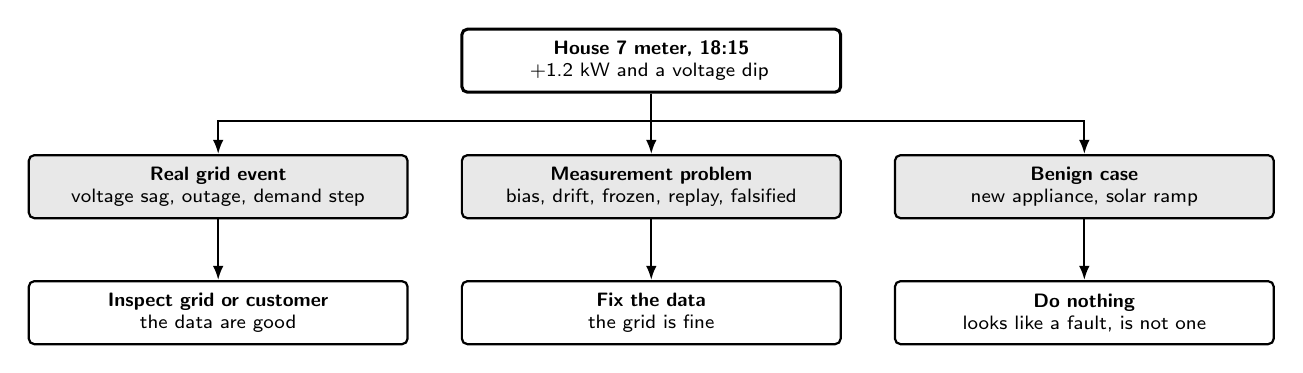
\begin{tikzpicture}
\node[box,line width=1.1pt,text width=4.6cm] (m) at (7.9,0) {\textbf{House 7 meter, 18:15}\\+1.2~kW and a voltage dip};
\node[gbox,text width=4.6cm] (a) at (2.4,-1.6) {\textbf{Real grid event}\\voltage sag, outage, demand step};
\node[gbox,text width=4.6cm] (b) at (7.9,-1.6) {\textbf{Measurement problem}\\bias, drift, frozen, replay, falsified};
\node[gbox,text width=4.6cm] (c) at (13.4,-1.6) {\textbf{Benign case}\\new appliance, solar ramp};
\node[box,text width=4.6cm] (a2) at (2.4,-3.2) {\textbf{Inspect grid or customer}\\the data are good};
\node[box,text width=4.6cm] (b2) at (7.9,-3.2) {\textbf{Fix the data}\\the grid is fine};
\node[box,text width=4.6cm] (c2) at (13.4,-3.2) {\textbf{Do nothing}\\looks like a fault, is not one};
\draw[arr] (m.south) -- ++(0,-0.35) -| (a.north);
\draw[arr] (m.south) -- (b.north);
\draw[arr] (m.south) -- ++(0,-0.35) -| (c.north);
\draw[arr] (a)--(a2); \draw[arr] (b)--(b2); \draw[arr] (c)--(c2);
\end{tikzpicture}
\caption{One deviation, three explanations. Each calls for a different response, so the cause must be established before any action.}
\end{figure}
Mixing them up is the costly error: ``repairing'' a real outage as if it were a sensor glitch hides it, and alarming on a new appliance trains operators to ignore alarms. Where physics cannot decide, the right answer is to say so and ask a human.

\subsection{Our answer}
The brief~\cite{brief} names the forces behind the problem: seasonal peaks, fast-growing renewables, more smart meters, more connected devices. As AI takes on more grid decisions, the question is whether it \textbf{can be trusted and who is accountable when it is wrong}. EnergyMind answers with a \textbf{trust layer} placed between raw data and automated action (Figure~\ref{fig:trust}). Each of its four functions corresponds to one goal of the challenge.

\begin{figure}[!h]
\centering
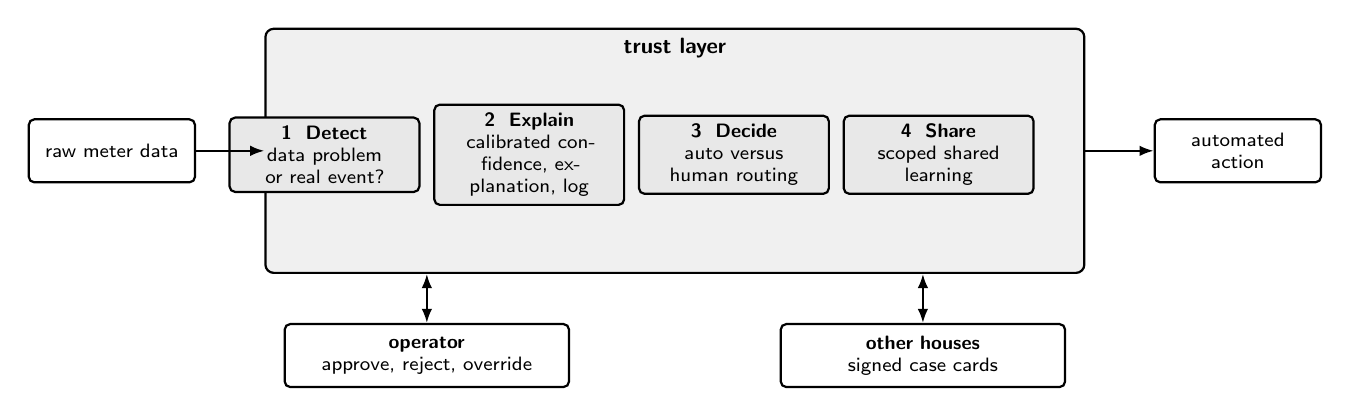
\begin{tikzpicture}
\node[box,text width=1.9cm] (raw) at (1.0,1.0) {raw meter data};
\node[box,text width=1.9cm] (act) at (15.3,1.0) {automated action};
\node[draw=black,thick,rounded corners=3pt,fill=black!6,minimum width=10.4cm,minimum height=3.1cm] (tl) at (8.15,1.0) {};
\node[font=\sffamily\bfseries\footnotesize] at (8.15,2.3) {trust layer};
\node[gbox,text width=2.2cm] (g1) at (3.7,0.95) {\textbf{1~~Detect}\\data problem or real event?};
\node[gbox,text width=2.2cm] (g2) at (6.3,0.95) {\textbf{2~~Explain}\\calibrated confidence, explanation, log};
\node[gbox,text width=2.2cm] (g3) at (8.9,0.95) {\textbf{3~~Decide}\\auto versus human routing};
\node[gbox,text width=2.2cm] (g4) at (11.5,0.95) {\textbf{4~~Share}\\scoped shared learning};
\node[box,text width=3.4cm] (op) at (5.0,-1.6) {\textbf{operator}\\approve, reject, override};
\node[box,text width=3.4cm] (ot) at (11.3,-1.6) {\textbf{other houses}\\signed case cards};
\draw[arr] (raw) -- (tl.west |- raw); \draw[arr] (tl.east |- act) -- (act);
\draw[barr] (op.north) -- (op.north |- tl.south);
\draw[barr] (ot.north) -- (ot.north |- tl.south);
\end{tikzpicture}
\caption{The trust layer sits between raw data and automated action. It decides whether the data may be used, says why and how sure it is, and decides who may act on that. The four numbered functions are the four challenge goals.}
\label{fig:trust}
\end{figure}
The report follows the Phase 1 brief: scope, objectives, data and anomaly-simulation plan, global architecture, then the design of each goal.

\section{Scope}
\label{sec:scope}
A reading can look wrong for two opposite reasons. A \textbf{data-quality problem} (a biased or drifting sensor, a frozen register, a replayed or falsified stream) calls for fixing the meter; the grid is fine. A \textbf{real grid event} (a voltage sag, an outage, a demand step) calls for inspecting the grid or the customer; the data are good. A third group, \textbf{benign cases} (a new appliance, a solar ramp), needs nothing.

Our slice of the energy system is \textbf{one smart-metered house, seen as a node}: voltage, current, power, power factor and an energy counter at one-minute resolution~\cite{brief}. \textbf{In this project, nodes are houses.} This is the data a utility already uses for billing, public datasets exist, and both faults and fraud matter. Three small experiments extend the node: a \textbf{feeder} (a house with its neighbours and an upstream meter), an \textbf{evidence fusion} test, and a \textbf{case-sharing} protocol between two houses.

\begin{table}[!h]
\small\centering
\caption{Scope boundaries.}
\begin{tabularx}{\textwidth}{@{}YY@{}}
\toprule
\hdr \textbf{In scope (Phase 1)} & \textbf{Out of scope}\\
\midrule
One house node covering the four goals; three small experiments & Real attack data; control of real equipment\\
Real recordings with a documented fault injector; a published synthetic dataset & Multi-site production deployment; federated learning\\
A deny-by-default policy, a tamper-evident log, an operator-interface prototype & Factories and microgrids: the design does not cover them\\
\bottomrule
\end{tabularx}
\end{table}

\section{Objectives}
\label{sec:objectives}
\begin{table}[!h]
\small\centering
\caption{Project objectives: the four goals as testable requirements.}
\begin{tabularx}{\textwidth}{@{}lYYl@{}}
\toprule
\hdr  & \textbf{Requirement} & \textbf{Measured by} & \textbf{Section}\\
\midrule
O1 & \textbf{Goal~1.} Separate normal data, measurement problems and real events; do not alarm on benign cases & Event-level precision and recall, false alarms per day & \ref{sec:goal1}\\
O2 & \textbf{Goal~2.} A calibrated confidence, a clear explanation (rules, SHAP, LIME), an auditable log & Calibration, evidence linked to each verdict & \ref{sec:goal2}\\
O3 & \textbf{Goal~3.} Explicit auto/human thresholds, an operator interface, safeguards against over- and under-trust & Policy tests & \ref{sec:goal3}\\
O4 & \textbf{Goal~4.} What is shared, what stays local, and why & Safety and privacy probes & \ref{sec:goal4}\\
O5 & Reproducible repository and open data & Seeded scripts, tests & \ref{app:repo}\\
\bottomrule
\end{tabularx}
\end{table}
\textbf{Principles:} say ``I cannot tell'' when physics cannot decide; never count an unevaluated check as passed; keep the policy independent of the model; audit our benchmark before trusting a number; report what did not work.

\clearpage
\section{Data and anomaly-simulation plan}
\label{sec:data}
Real grid data labelled with faults is rare, so the brief expects simulation: start from realistic data and inject documented faults~\cite{brief}.

\subsection{The data: what we reviewed and what we chose}
We reviewed many open datasets. In the end we kept \textbf{WPuQ, AMPds2 and SimBench} to build our published dataset. To develop and test detection we also used the ECO recordings; ECO is not part of the published dataset.
\begin{table}[!h]
\small\centering
\caption{Datasets we kept.}
\begin{tabularx}{\textwidth}{@{}lYY@{}}
\toprule
\hdr \textbf{Source} & \textbf{Content} & \textbf{Use}\\
\midrule
WPuQ~\cite{wpuq} & German houses, real three-phase load curves & Load shapes and meter model of the published dataset; one fusion test\\
AMPds2~\cite{ampds} & One Canadian house, two years, appliances metered one by one & Appliance profiles of the published dataset; second detection domain\\
SimBench~\cite{simbench} & Simulated low-voltage grids (calculations with pandapower~\cite{pandapower}) & Grid of the published dataset; feeder experiment\\
ECO~\cite{eco} & 6 Swiss houses, measurements every second & Development and tests of detection only\\
\bottomrule
\end{tabularx}
\end{table}
Other sources (real UK solar production, STEG statistics, the PVGIS solar resource~\cite{pvgis}) were reviewed and are planned for Phase 2. No dataset is Tunisian. Also, some datasets compute quantities from others (for example apparent power); the matching checks can then never fail. We mark them ``not evaluable'' and never count them as passed.

\subsection{The published dataset}
\label{sec:dataset}
The dataset is available on Kaggle: \url{\HFURL}. It is a validated baseline for a neighbourhood of 13 smart-metered houses, with two views of every house: \emph{ground\_truth} (true values from a three-phase grid calculation) and \emph{measured} (what a meter would report, with the gain error and noise of a real WPuQ meter).
\begin{quote}\small
\textbf{Important:} no anomaly has been injected into the \emph{measured} view yet. It contains only the normal noise of a meter. The injection, described below, is the next step.
\end{quote}
\begin{figure}[!h]
\centering
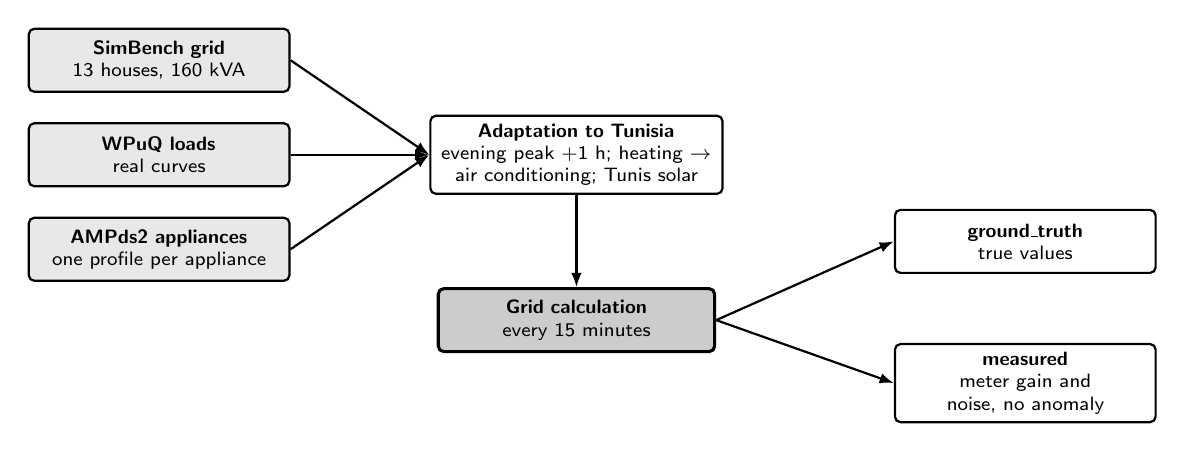
\begin{tikzpicture}
\node[gbox,text width=3.1cm] (s1) at (1.9,2.7) {\textbf{SimBench grid}\\13 houses, 160~kVA};
\node[gbox,text width=3.1cm] (s2) at (1.9,1.5) {\textbf{WPuQ loads}\\real curves};
\node[gbox,text width=3.1cm] (s3) at (1.9,0.3) {\textbf{AMPds2 appliances}\\one profile per appliance};
\node[box,text width=3.5cm] (ad) at (7.2,1.5) {\textbf{Adaptation to Tunisia}\\evening peak +1~h; heating $\to$ air conditioning; Tunis solar};
\node[hbox,text width=3.3cm] (pf) at (7.2,-0.6) {\textbf{Grid calculation}\\every 15 minutes};
\node[box,text width=3.1cm] (gt) at (12.9,0.4) {\textbf{ground\_truth}\\true values};
\node[box,text width=3.1cm] (me) at (12.9,-1.4) {\textbf{measured}\\meter gain and noise, no anomaly};
\foreach \s in {s1,s2,s3} {\draw[arr] (\s.east) -- (ad.west);}
\draw[arr] (ad.south) -- (pf.north);
\draw[arr] (pf.east) -- (gt.west); \draw[arr] (pf.east) -- (me.west);
\end{tikzpicture}
\caption{Construction of the published dataset (seeded, one command).}
\end{figure}
\begin{table}[!h]
\small\centering
\caption{The published dataset at a glance.}
\begin{tabularx}{\textwidth}{@{}lY@{}}
\toprule
\hdr \textbf{Property} & \textbf{Value}\\
\midrule
Content & 13 houses, one 160~kVA transformer, one year (2018) every 15 minutes; 32 columns: voltage, current, power and power factor per phase, solar output, power per appliance\\
Validation & 14 physical checks pass: converging calculations, voltages within $\pm$10\,\% (EN~50160~\cite{en50160}), transformer loading at most 66.6\,\%, energy balances close\\
Licence and limits & Open Database License~\cite{odbl}; synthetic, a single topology, 2018 calendar\\
\bottomrule
\end{tabularx}
\end{table}

\subsection{Anomaly-simulation plan}
\label{sec:injection}
The injector (\code{energymind/inject.py}, seeded) adds incidents of three classes. A \textbf{measurement problem} changes only what the meter reports, so physical relations break. A \textbf{real event} changes the state of the grid consistently, so relations hold. A \textbf{benign case} has the same physics as a demand step and stays labelled normal. Three severities (0.3, 0.6, 1.0) scale each effect.
\begin{table}[!h]
\small\centering
\caption{The 16 injected anomaly subtypes, in plain words.}
\begin{tabularx}{\textwidth}{@{}l l Y l@{}}
\toprule
\hdr \textbf{Class} & \textbf{Subtype} & \textbf{Effect} & \textbf{Duration}\\
\midrule
Measurement & \code{bias}, \code{drift} & constant offset, or one that grows gradually (up to 8\,\%) & 30--180 min\\
 & \code{scale}, \code{noise} & reading multiplied by a factor; noise added & 20--120 min\\
 & \code{frozen}, \code{dropout} & value held; missing data & 10--90 min\\
 & \code{delay}, \code{replay} & delayed values; values of an earlier day replayed & 30--120 min\\
 & \code{falsified} & current and powers lowered together, voltage unchanged & 60--180 min\\
Real event & \code{voltage_sag}, \code{outage} & voltage lowered; almost total loss of supply & 10--120 min\\
 & \code{demand_step}, \code{duty_cycle}, \code{phase_imbalance} & load rises; square-wave load; unbalanced phases & 30--180 min\\
Benign & \code{benign_new_load}, \code{benign_pv_ramp} & new appliance; smooth solar variation & 60--180 min\\
\bottomrule
\end{tabularx}
\end{table}
\textbf{Rules.} The input is never modified; two incidents per day on average; incidents never overlap and stay 60 minutes from split edges; the ground truth never reaches a model or the policy at inference. \textbf{Limits:} events are bounded and revert to normal; \code{falsified}, \code{demand_step} and benign cases can be told apart only by context (time of day, history, a second meter).

\textbf{Current status.} The injector has been run on the real recordings, and the detection of Goal~1 was tested on them. \textbf{Next step (Phase 2):} inject these anomalies into the \emph{measured} view of the published dataset, with their labels, and rerun detection there.

\clearpage
\section{Global architecture}
\label{sec:arch}
The system is built around \textbf{one node = one house}. Each node contains the trust layer, which receives the meter's measurements, analyses them, takes a decision and can share a lesson with other houses. Services above the nodes (a feeder service and a city coordinator) group houses by feeder and route incidents; the neighbourhood only defines scope. Figure~\ref{fig:arch-simple} is the simple view; Figure~\ref{fig:arch-detail} adds the services and the tools of the target design.

\begin{figure}[!h]
\centering
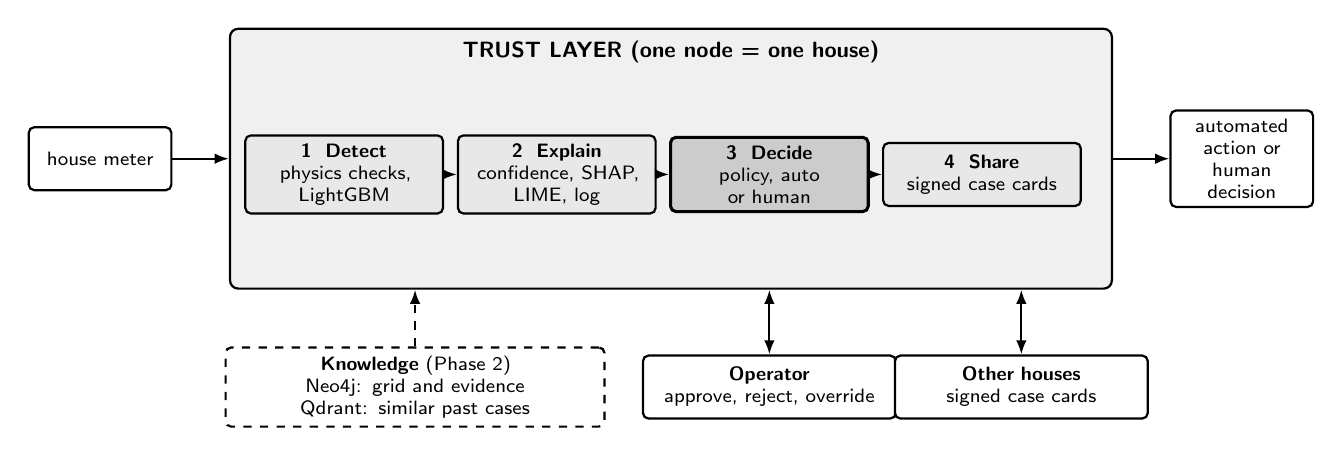
\begin{tikzpicture}
\node[box,text width=1.6cm] (src) at (0.9,1.2) {house meter};
\node[box,text width=1.6cm] (act) at (15.4,1.2) {automated action or human decision};
\node[draw=black,thick,rounded corners=3pt,fill=black!6,minimum width=11.2cm,minimum height=3.3cm] (tl) at (8.15,1.2) {};
\node[font=\sffamily\bfseries\footnotesize] at (8.15,2.55) {TRUST LAYER (one node = one house)};
\node[gbox,text width=2.3cm] (m1) at (4.0,1.0) {\textbf{1~~Detect}\\physics checks, LightGBM};
\node[gbox,text width=2.3cm] (m2) at (6.7,1.0) {\textbf{2~~Explain}\\confidence, SHAP, LIME, log};
\node[hbox,text width=2.3cm] (m3) at (9.4,1.0) {\textbf{3~~Decide}\\policy, auto or human};
\node[gbox,text width=2.3cm] (m4) at (12.1,1.0) {\textbf{4~~Share}\\signed case cards};
\draw[arr] (m1)--(m2); \draw[arr] (m2)--(m3); \draw[arr] (m3)--(m4);
\draw[arr] (src) -- (tl.west |- src); \draw[arr] (tl.east |- act) -- (act);
\node[box,text width=3.0cm] (op) at (9.4,-1.7) {\textbf{Operator}\\approve, reject, override};
\node[box,text width=3.0cm] (ot) at (12.6,-1.7) {\textbf{Other houses}\\signed case cards};
\node[dbox,text width=4.6cm] (kn) at (4.9,-1.7) {\textbf{Knowledge} (Phase 2)\\Neo4j: grid and evidence\\Qdrant: similar past cases};
\draw[barr] (op.north) -- (op.north |- tl.south);
\draw[barr] (ot.north |- tl.south) -- (ot.north);
\draw[darr] (kn.north) -- (kn.north |- tl.south);
\end{tikzpicture}
\caption{Simple view of the architecture. Solid boxes: Phase 1 prototype. Dashed boxes: Phase 2 design.}
\label{fig:arch-simple}
\end{figure}

\begin{figure}[!h]
\centering
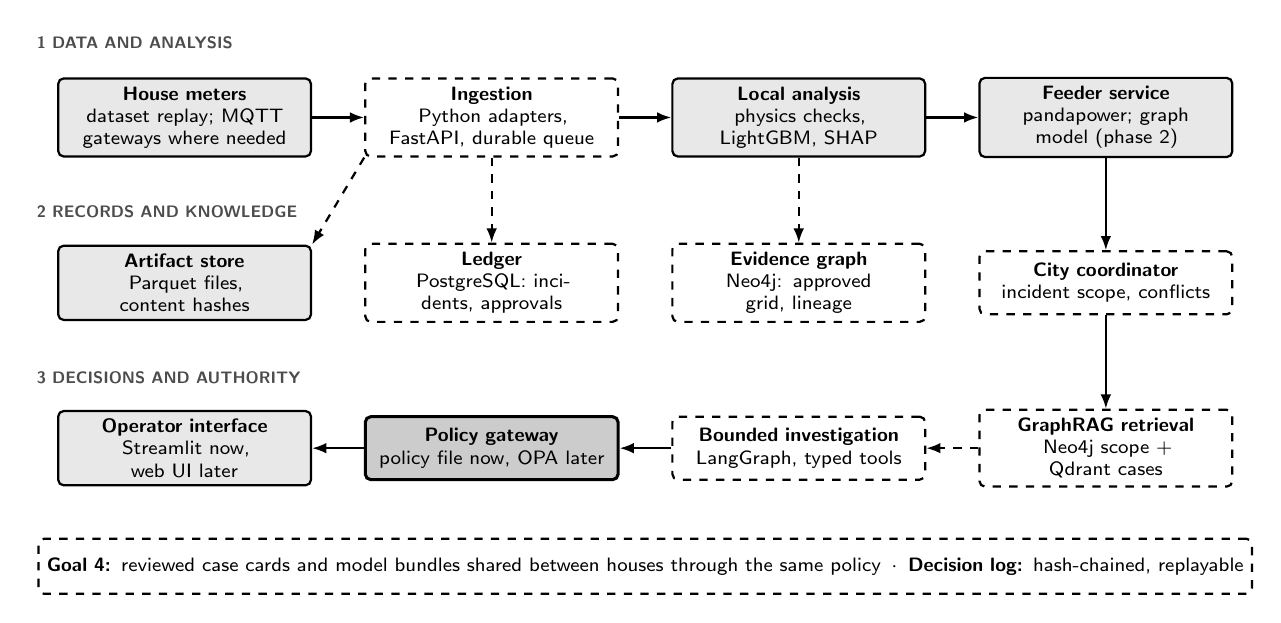
\begin{tikzpicture}
\node[tag,anchor=west] at (-0.3,4.4) {1  DATA AND ANALYSIS};
\node[gbox,text width=3.0cm] (src) at (1.7,3.45) {\textbf{House meters}\\dataset replay; MQTT gateways where needed};
\node[dbox,text width=3.0cm] (ing) at (5.6,3.45) {\textbf{Ingestion}\\Python adapters, FastAPI, durable queue};
\node[gbox,text width=3.0cm] (loc) at (9.5,3.45) {\textbf{Local analysis}\\physics checks, LightGBM, SHAP};
\node[gbox,text width=3.0cm] (fed) at (13.4,3.45) {\textbf{Feeder service}\\pandapower; graph model (phase 2)};
\draw[arr] (src)--(ing); \draw[arr] (ing)--(loc); \draw[arr] (loc)--(fed);
\node[tag,anchor=west] at (-0.3,2.25) {2  RECORDS AND KNOWLEDGE};
\node[gbox,text width=3.0cm] (art) at (1.7,1.35) {\textbf{Artifact store}\\Parquet files, content hashes};
\node[dbox,text width=3.0cm] (led) at (5.6,1.35) {\textbf{Ledger}\\PostgreSQL: incidents, approvals};
\node[dbox,text width=3.0cm] (gr) at (9.5,1.35) {\textbf{Evidence graph}\\Neo4j: approved grid, lineage};
\node[dbox,text width=3.0cm] (cc) at (13.4,1.35) {\textbf{City coordinator}\\incident scope, conflicts};
\draw[darr] (ing.south west) -- (art.north east); \draw[darr] (ing.south)--(led.north); \draw[darr] (loc.south)--(gr.north); \draw[arr] (fed.south)--(cc.north);
\node[tag,anchor=west] at (-0.3,0.15) {3  DECISIONS AND AUTHORITY};
\node[dbox,text width=3.0cm] (ret) at (13.4,-0.75) {\textbf{GraphRAG retrieval}\\Neo4j scope + Qdrant cases};
\node[dbox,text width=3.0cm] (inv) at (9.5,-0.75) {\textbf{Bounded investigation}\\LangGraph, typed tools};
\node[hbox,text width=3.0cm] (pol) at (5.6,-0.75) {\textbf{Policy gateway}\\policy file now, OPA later};
\node[gbox,text width=3.0cm] (op) at (1.7,-0.75) {\textbf{Operator interface}\\Streamlit now, web UI later};
\draw[arr] (cc.south)--(ret.north); \draw[darr] (ret)--(inv); \draw[arr] (inv)--(pol); \draw[arr] (pol)--(op);
\node[box,dashed,text width=15.2cm,minimum height=7mm] at (7.55,-2.25) {\textbf{Goal 4:} reviewed case cards and model bundles shared between houses through the same policy \,$\cdot$\, \textbf{Decision log:} hash-chained, replayable};
\end{tikzpicture}
\caption{Detailed view: services and tools. Solid boxes exist in the Phase 1 prototype (the feeder is an experiment, not wired into the node pipeline); dashed boxes are the Phase 2 design.}
\label{fig:arch-detail}
\end{figure}

\begin{table}[!h]
\small\centering
\caption{Components, tools and status. We start with the smallest set and add a tool only when a measured need justifies it.}
\begin{tabularx}{\textwidth}{@{}lYYl@{}}
\toprule
\hdr \textbf{Component} & \textbf{Target tool, and why} & \textbf{Phase 1 stand-in} & \textbf{Phase}\\
\midrule
Data and numerics & Python, pandas, Parquet: simple, reproducible & Same & 1\\
Grid physics & pandapower, SimBench: open source, standard for distribution grids & Same & 1\\
Detection & LightGBM, scikit-learn (PyTorch for one baseline): fast and accurate on tabular data & Same & 1\\
Explanations & SHAP (exact for trees) and LIME (model-independent second opinion): named by the brief & SHAP only & 1, 2\\
Operator interface & Streamlit now; an authenticated web interface later & Streamlit prototype & 1, 2\\
Service interfaces & FastAPI: typed, versioned messages & Scripts & 2\\
Operational ledger & PostgreSQL: incidents, approvals, pending events & Hash-chained JSONL log & 2\\
Grid and evidence graph & Neo4j: ``who is connected to whom'' is a graph~\cite{neo4jrag} & pandapower network & 2\\
Past-case search & Qdrant: fast similarity search with filters~\cite{qdrant} & JSON cards, nearest neighbour & 2\\
Investigation workflow & LangGraph: durable states, human checkpoints~\cite{langgraph} & None & 2\\
Policy engine & OPA: rules kept outside the code~\cite{opa} & Policy file (YAML) & 2\\
Packaging & Docker Compose on one workstation; a message broker only at city scale & Virtual environment & 2\\
\bottomrule
\end{tabularx}
\end{table}

\textbf{Four rules hold everywhere.} (1) No language model on the detection path. (2) Detection continues even if retrieval or text writing fails. (3) Every explanation has a template fallback. (4) The authority to act comes from a policy that no model output can override.

\textbf{From a measurement to committed evidence.} An adapter validates the schema, units, phase and timestamps of a measurement and keeps the raw bytes by content hash; normalisation never overwrites the source. A window builder writes a versioned manifest, and the object, the manifest and a pending event are committed together, so an event is published only once the window is ready. Late data creates a new evidence version, never an edit of a decision's inputs. A projection worker then writes typed projections into \textbf{Neo4j} (grid, evidence, lineage) through parameterised transactions; no sample is stored as a graph node, and a language model cannot invent assets or arbitrary queries. Every observation carries a lineage identifier, so five residuals computed from one meter do not count as five confirmations. A \textbf{replay trace} links one incident end to end (Section~\ref{sec:goal3}).

\textbf{Interfaces and events.} Services exchange typed, versioned messages; mutations carry an idempotency key, long jobs return a job identifier, and an unsupported check is a typed result, never a hidden failure.
\begin{table}[!h]
\small\centering
\caption{Main events of the target design.}
\begin{tabularx}{\textwidth}{@{}lYY@{}}
\toprule
\hdr \textbf{Event} & \textbf{Consumers} & \textbf{Rule}\\
\midrule
\texttt{measurement.window.ready} & Local analysis & Artifact and manifest committed; no labels\\
\texttt{local.evidence.ready} & Feeder service, graph projection & Check results with exact model and grid versions\\
\texttt{incident.updated} & Investigation, interface & Monotonic incident version; contradictions kept\\
\texttt{decision.recorded} & Interface, executor, audit & Independent policy and action authority\\
\texttt{case.approved}, \texttt{case.revoked} & Graph and vector indexers & The review scope is authoritative\\
\bottomrule
\end{tabularx}
\end{table}

\clearpage
\section{Goal 1: anomaly and bias detection}
\label{sec:goal1}
\goalbadge{GOAL 1} The system must detect equipment faults, degraded sensors, and biased, corrupted or falsified readings, and distinguish a real grid event from a data-quality problem~\cite{brief}. The tested models and the curves of this report are all in this section.

\subsection{Architecture of Goal 1}
\begin{figure}[!h]
\centering
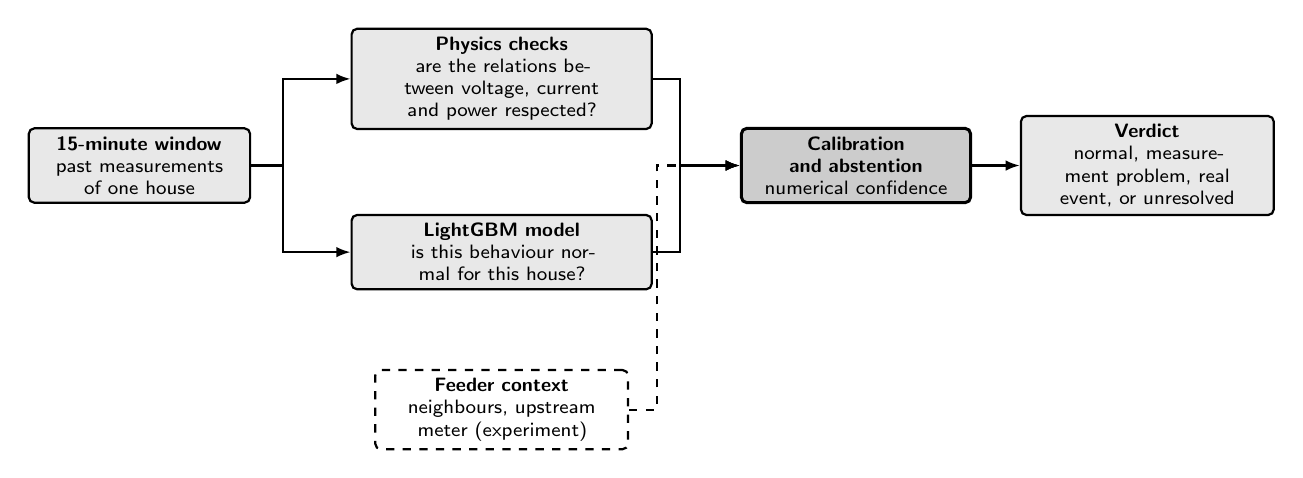
\begin{tikzpicture}
\node[gbox,text width=2.6cm] (w) at (1.6,0.6) {\textbf{15-minute window}\\past measurements of one house};
\node[gbox,text width=3.6cm] (b1) at (6.2,1.7) {\textbf{Physics checks}\\are the relations between voltage, current and power respected?};
\node[gbox,text width=3.6cm] (b2) at (6.2,-0.5) {\textbf{LightGBM model}\\is this behaviour normal for this house?};
\node[dbox,text width=3.0cm] (b3) at (6.2,-2.5) {\textbf{Feeder context}\\neighbours, upstream meter (experiment)};
\node[hbox,text width=2.7cm] (ca) at (10.7,0.6) {\textbf{Calibration and abstention}\\numerical confidence};
\node[gbox,text width=3.0cm] (v) at (14.4,0.6) {\textbf{Verdict}\\normal, measurement problem, real event, or unresolved};
\draw[arr] (w.east) -- ++(0.4,0) |- (b1.west); \draw[arr] (w.east) -- ++(0.4,0) |- (b2.west);
\draw[arr] (b1.east) -- ++(0.35,0) |- (ca.west); \draw[arr] (b2.east) -- ++(0.35,0) |- (ca.west);
\draw[darr] (b3.east) -- ++(0.35,0) |- (ca.west);
\draw[arr] (ca)--(v);
\end{tikzpicture}
\caption{Architecture of Goal~1. Detector v1 combines the physics checks and the model in one LightGBM model; the feeder context is a separate experiment.}
\end{figure}

\textbf{Principle.} A healthy meter respects a few physical relations (for example, apparent power equals voltage times current). A faulty sensor often breaks one of them; a real grid event respects them all, because the electrical state really changed. The detector therefore computes \emph{residuals} (the gaps to these relations), plus the length of frozen values, the share of missing data, variation statistics, and context (time of day, history from 60 minutes to 7 days). A check that cannot be evaluated is flagged, never counted as passed.

\subsection{Method and evaluation protocol}
\textbf{Detector v1.} A 15-minute window (stride 5), built only from past measurements, is classified by a LightGBM model~\cite{lightgbm} (three classes: normal, measurement problem, real event), then its confidence is calibrated by temperature scaling~\cite{guo}. A window raises an alert if its ``abnormal'' probability exceeds a threshold chosen on a validation slice; neighbouring alerts are merged into segments. We compare with five baselines: a robust $z$-score, Isolation Forest, One-Class SVM, a causal convolutional network (TCN) and an autoencoder.

\textbf{Protocol.} Per-window scores are inflated by correlated neighbouring windows, and ``point adjustment'' overstates detection~\cite{tatbul}. We therefore score \textbf{per event}: an alert matches an incident if it overlaps it within $\pm$15 minutes; we compute precision and recall per class, the \textbf{event macro-F1} (mean of the two fault classes) and \textbf{false alarms per day (FA/day)}. The split is by time (60\,\% training, 15\,\% calibration, 25\,\% test, with a 60-minute purge), and whole houses are held out.

\textbf{We audited our own benchmark.} The first injector modified channels that the loader computes from others without recomputing them: measurement faults produced impossible residuals, and a clue made it possible to guess the label (AUC 0.999). Injector v2 modifies only real registers; the AUC fell to 0.500 and permutation tests give chance level. The numbers went down (baseline window F1: 0.724 then 0.566; false alarms: 2.12 then 7.15 per day), but the conclusions are now defensible.

\subsection{Results on the corrected benchmark}
\begin{table}[!h]
\footnotesize\centering
\caption{Detector v1 against the baseline (LightGBM), per event. P/R = precision/recall. Synthetic faults on real data.}
\begin{tabularx}{\textwidth}{@{}llCCCC@{}}
\toprule
\hdr \textbf{Scenario} & \textbf{Model} & \textbf{Measurement P / R} & \textbf{Real event P / R} & \textbf{Macro-F1} & \textbf{FA/day}\\
\midrule
Training houses & baseline & 0.242 / 0.797 & 0.144 / 0.795 & 0.307 & 7.27\\
 & \textbf{v1} & 0.843 / 0.772 & 0.974 / 0.631 & \textbf{0.786} & 0.144\\
Held-out house 1 & baseline & 0.148 / 0.972 & 0.545 / 0.287 & 0.317 & 6.28\\
 & \textbf{v1} & 0.423 / 0.808 & 0.943 / 0.465 & \textbf{0.589} & 0.971\\
Held-out house 2 & baseline & 0.278 / 0.824 & 0.259 / 0.658 & 0.393 & 3.54\\
 & \textbf{v1} & 0.574 / 0.705 & 0.727 / 0.491 & \textbf{0.609} & 0.533\\
AMPds2 & baseline & 0.151 / 0.910 & 0.208 / 0.815 & 0.295 & 7.85\\
 & \textbf{v1} & 0.785 / 0.605 & 0.900 / 0.664 & \textbf{0.724} & 0.212\\
WPuQ (indicative) & \textbf{v1} & 0.882 / 0.827 & 0.667 / 0.690 & \textbf{0.766} & 0.253\\
\bottomrule
\end{tabularx}
\end{table}

\begin{figure}[!h]
\centering
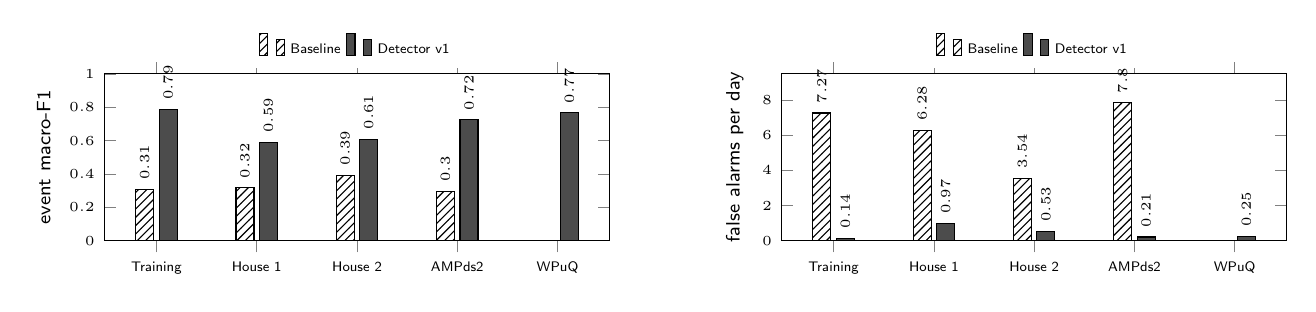
\begin{tikzpicture}
\begin{axis}[ybar,bar width=6.5pt,width=8.0cm,height=3.7cm,ymin=0,ymax=1.0,
 symbolic x coords={inhouse,eco03,eco06,ampds,wpuq},xtick={inhouse,eco03,eco06,ampds,wpuq},
 xticklabels={Training,House 1,House 2,AMPds2,WPuQ},
 x tick label style={font=\sffamily\tiny},y tick label style={font=\sffamily\tiny},
 ylabel={event macro-F1},ylabel style={font=\sffamily\scriptsize},enlarge x limits=0.13,
 nodes near coords,every node near coord/.append style={font=\sffamily\tiny,rotate=90,anchor=west,/pgf/number format/.cd,fixed,precision=2},
 legend style={font=\sffamily\tiny,at={(0.5,1.03)},anchor=south,legend columns=2,draw=none}]
\addplot[fill=white,draw=black,pattern=north east lines] coordinates {(inhouse,0.307) (eco03,0.317) (eco06,0.393) (ampds,0.295)};
\addplot[fill=black!70,draw=black] coordinates {(inhouse,0.786) (eco03,0.589) (eco06,0.609) (ampds,0.724) (wpuq,0.766)};
\legend{Baseline,Detector v1}
\end{axis}
\begin{axis}[at={(8.6cm,0)},ybar,bar width=6.5pt,width=8.0cm,height=3.7cm,ymin=0,ymax=9.5,
 symbolic x coords={inhouse,eco03,eco06,ampds,wpuq},xtick={inhouse,eco03,eco06,ampds,wpuq},
 xticklabels={Training,House 1,House 2,AMPds2,WPuQ},
 x tick label style={font=\sffamily\tiny},y tick label style={font=\sffamily\tiny},
 ylabel={false alarms per day},ylabel style={font=\sffamily\scriptsize},enlarge x limits=0.13,
 nodes near coords,every node near coord/.append style={font=\sffamily\tiny,rotate=90,anchor=west,/pgf/number format/.cd,fixed,precision=2},
 legend style={font=\sffamily\tiny,at={(0.5,1.03)},anchor=south,legend columns=2,draw=none}]
\addplot[fill=white,draw=black,pattern=north east lines] coordinates {(inhouse,7.27) (eco03,6.28) (eco06,3.54) (ampds,7.85)};
\addplot[fill=black!70,draw=black] coordinates {(inhouse,0.144) (eco03,0.971) (eco06,0.533) (ampds,0.212) (wpuq,0.253)};
\legend{Baseline,Detector v1}
\end{axis}
\end{tikzpicture}
\caption{Event macro-F1 (left, higher is better) and false alarms per day (right, lower is better). WPuQ has no baseline and is indicative.}
\end{figure}

\textbf{The price of precision.} Detector v1 is an operating point that favours precision. Recall of three fault types collapses (\code{demand_step} 0.111; \code{duty_cycle} 0.086; \code{falsified} 0.029, against 0.63; 0.57; 0.23 before); the median delay rises from 2 to 10 minutes; in return, benign cases that raise an alarm drop from 66\,\% to 2\,\%. On unseen houses the F1 loses about 0.2. \code{falsified} respects every physical relation by construction: it is detected (0.743) but rarely classified correctly (0.343).

\begin{figure}[!h]
\centering
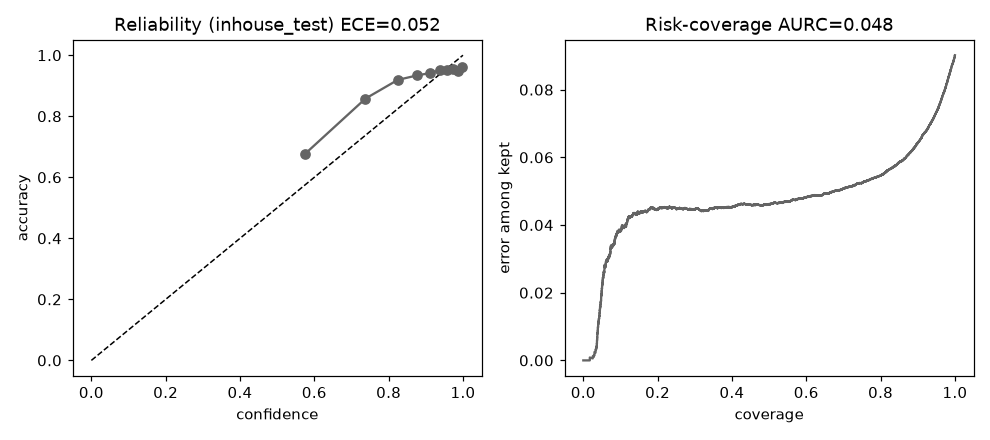
\includegraphics[width=0.5\textwidth]{figures/reliability.png}
\caption{Calibration of detector v1 on the training houses (calibration error 0.052): reliability diagram (left) and risk--coverage curve (right). Abstaining below 0.55 confidence cuts the baseline's false alarms from 7.15 to 1.92 per day, at the cost of lower recall (0.926 then 0.784).}
\end{figure}

\begin{table}[!h]
\small\centering
\caption{Baseline models on the training houses (window macro-F1; recall measurement / real event; p95 inference time per call on a laptop CPU, not a load test).}
\begin{tabularx}{\textwidth}{@{}lCCCCC@{}}
\toprule
\hdr \textbf{Model} & \textbf{Macro-F1} & \textbf{Recall} & \textbf{FA/day} & \textbf{Calib.} & \textbf{p95 (ms)}\\
\midrule
Robust $z$-score & 0.436 & 0.917 / 0.881 & 6.09 & 0.458 & 0.24\\
Isolation Forest & 0.432 & 0.946 / 0.938 & 8.45 & 0.223 & 14.30\\
One-Class SVM & 0.436 & 0.946 / 0.960 & 9.49 & 0.208 & 1.03\\
LightGBM & 0.566 & 0.934 / 0.926 & 7.15 & 0.076 & 1.79\\
Causal TCN (3 seeds) & 0.535 & 0.322 / 0.398 & 0.08 & 0.010 & 4.12\\
Convolutional autoencoder & -- & 0.174 / 0.040 & 0.05 & 0.012 & 0.74\\
\bottomrule
\end{tabularx}
\end{table}
LightGBM is the best baseline; the TCN is cautious and does not beat it. Without the physics residuals, the macro-F1 drops to 0.453. \textbf{Transfer from one dataset to another fails:} from ECO to AMPds2 without adaptation, LightGBM reaches 0.476 (0.613 on site); a per-house adaptation step is needed.

\textbf{Feeder context and fusion.} On a SimBench feeder, neighbouring and upstream meters add 4.1 points of event accuracy on the same feeder (95\,\% confidence interval 1.6 to 6.5) and 7.3 points on another feeder (4.9 to 9.9). Eight detectors reading the same meter are not eight confirmations: naive fusion becomes badly over-confident (confidence minus accuracy up to $+0.907$); fusion that accounts for provenance brings it back to $-0.017$ without improving accuracy. We report this negative result.

\textbf{Next steps (Phase 2).} Three extensions, each kept only if it beats a simpler model: \textbf{appliance-level consumption estimation} (NILM, causal TCN~\cite{seq2point}), \textbf{richer physics checks} (feeder balance, circuit model) and a \textbf{graph model} using relations between neighbouring houses.

\clearpage
\section{Goal 2: confidence and explainability}
\label{sec:goal2}
\goalbadge{GOAL 2} Every flagged event must come with a verdict a human can understand and verify: a confidence score, a plain-language explanation and an auditable log of what was detected, concluded and why. The brief encourages interpretable approaches (SHAP, LIME, rule-backed models) and asks to avoid black boxes~\cite{brief}.

\subsection{Architecture of Goal 2}
\begin{figure}[!h]
\centering
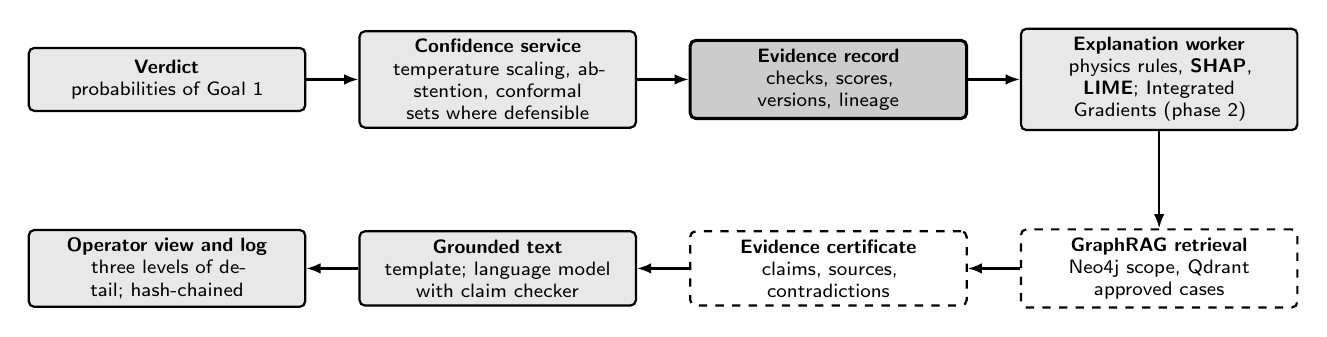
\begin{tikzpicture}
\node[gbox,text width=3.3cm] (v) at (1.9,2.6) {\textbf{Verdict}\\probabilities of Goal~1};
\node[gbox,text width=3.3cm] (c) at (6.1,2.6) {\textbf{Confidence service}\\temperature scaling, abstention, conformal sets where defensible};
\node[hbox,text width=3.3cm] (e) at (10.3,2.6) {\textbf{Evidence record}\\checks, scores, versions, lineage};
\node[gbox,text width=3.3cm] (x) at (14.5,2.6) {\textbf{Explanation worker}\\physics rules, \textbf{SHAP}, \textbf{LIME}; Integrated Gradients (phase 2)};
\draw[arr] (v)--(c); \draw[arr] (c)--(e); \draw[arr] (e)--(x);
\node[dbox,text width=3.3cm] (r) at (14.5,0.2) {\textbf{GraphRAG retrieval}\\Neo4j scope, Qdrant approved cases};
\node[dbox,text width=3.3cm] (k) at (10.3,0.2) {\textbf{Evidence certificate}\\claims, sources, contradictions};
\node[gbox,text width=3.3cm] (g) at (6.1,0.2) {\textbf{Grounded text}\\template; language model with claim checker};
\node[gbox,text width=3.3cm] (o) at (1.9,0.2) {\textbf{Operator view and log}\\three levels of detail; hash-chained};
\draw[arr] (x)--(r); \draw[arr] (r)--(k); \draw[arr] (k)--(g); \draw[arr] (g)--(o);
\end{tikzpicture}
\caption{Architecture of Goal~2. Dashed boxes are the Phase 2 design. The text can never add a number, a meter or a cause that is absent from the evidence.}
\end{figure}

\subsection{Confidence, abstention and action risk}
Confidence is the calibrated probability of the predicted class: a model that announces 80\,\% should be right about 8 times out of 10 (calibration error 0.052 on the training houses). We report \emph{four separate quantities}, not one score.
\begin{table}[!h]
\small\centering
\caption{The four components of confidence.}
\begin{tabularx}{\textwidth}{@{}lYY@{}}
\toprule
\hdr \textbf{Component} & \textbf{Question} & \textbf{Method}\\
\midrule
Surprise & Is this unusual under normal operation? & Residuals compared with a clean reference\\
Cause & Which cause is most plausible? & Calibrated probabilities (temperature scaling); a prediction set where conformal methods~\cite{gibbs} are defensible\\
Localisation & Which meter and phase? & Share of the evidence attributed to each meter\\
Inputs & Can the inputs be trusted? & Missing share, unavailable checks\\
\bottomrule
\end{tabularx}
\end{table}
Below 0.55 confidence, or if the top two classes are too close, the system answers \emph{unresolved} and hands over to a human. \textbf{Confidence and action risk stay separate:} a confidence that justifies flagging a reading does not justify recalibrating a meter, and a quiet or unavailable check is never proof of normality.

\subsection{Explanations: rules, SHAP and LIME}
The brief explicitly names SHAP, LIME and rule-backed models as ways to explain a verdict without a black box, so we use them as complementary levels. \textbf{Physics rules} explain the \emph{physical why}; SHAP and LIME explain the \emph{behaviour of the model}. We put the rules first, because a model attribution is not proof of a physical cause. An asynchronous \textbf{explanation worker} runs after the numerical decision, loads the frozen model and the original features, and stores an \textbf{explanation artifact} (model run, target output, method and version, baseline or background, fidelity and stability measures, limits, input hash); detection continues if explanation fails.
\begin{table}[!h]
\small\centering
\caption{Explanation methods and how to read them.}
\begin{tabularx}{\textwidth}{@{}lYYl@{}}
\toprule
\hdr \textbf{Method} & \textbf{What it provides} & \textbf{Caution} & \textbf{Phase}\\
\midrule
Physics rules & Which relation is violated, with observed and expected values; names the checks that cannot be evaluated & Valid only where the instrumentation supports the check & 1\\
SHAP~\cite{treeshap} & Which variables weighed in the decision; exact for tree models such as LightGBM & Relative to a stated background; not a physical cause & 1\\
LIME~\cite{lime} & A simple model fitted around one decision: a second, model-independent opinion & Perturbations must stay physically valid; check stability & 2\\
Integrated Gradients~\cite{ig} & Attribution for the temporal model (TCN) along a path from a baseline & Zero voltage is a poor baseline; use a physically meaningful one & 2\\
Graph explainer~\cite{gnnexpl} & Important features, nodes and edges of a graph-model decision & Only after compatibility checks & 2\\
\bottomrule
\end{tabularx}
\end{table}

\subsection{Grounded knowledge: Neo4j, Qdrant and GraphRAG (Phase 2)}
Two stores play two different roles. \textbf{Neo4j} is the authoritative typed store of the approved grid, ownership, incidents, check lineage, decisions and approvals. \textbf{Qdrant} is an index over approved case and procedure representations only (a text vector from a multilingual encoder~\cite{e5}, a lexical vector and a numerical signature of the incident); numerical traces stay in the artifact store. Retrieval then follows five steps~\cite{neo4jrag,qdrant}: (1) resolve the incident's authorised part of the grid in Neo4j; (2) filter the Qdrant candidates by scope, equipment, feature schema, review status and validity; (3) retrieve the three representations separately and merge the ranks; (4) check compatibility in the graph; (5) return an \textbf{evidence certificate}, a small structured packet of claims, sources, contradictions and expiry. A similarity score is neither an electrical distance nor a probability, and a past case never overrides a fresh, contradicting measurement.

\textbf{Grounded writing.} A language model, if used, receives only the certificate; it may explain it or propose an approved check but cannot invent a measured value, a confidence or an identifier. A checker verifies every number and asset against the evidence, and the deterministic template remains the fallback. A local instruction-tuned model~\cite{qwen} and the multilingual encoder are candidates, to be tested on French, Arabic and English technical text; neither supplies confidence or authority. Explanation quality will be judged by fidelity, stability, agreement with the injected ground truth, and usefulness to operators.

\subsection{Log and Phase 1 prototype}
For each detection the prototype produces an \emph{evidence record} (probabilities, checks passed, failed or not evaluated, SHAP variables, versions) and a template explanation, for example: \emph{``Real event, confidence 80\,\%. Check passed: $p\le s$; the other relations are true by construction and cannot fail. Alternative explanation: a coordinated reporting error that keeps the relations consistent.''} Each log entry contains the hash of the previous one~\cite{crosby}; the human decision is appended, with a mandatory reason for a rejection or an override. A test confirms that editing or deleting an entry breaks verification (deleting the last entries needs an external anchor).

\clearpage
\section{Goal 3: human--AI escalation and governance}
\label{sec:goal3}
\goalbadge{GOAL 3} The system must define what the AI can do on its own and when a human must decide: thresholds for automatic corrective actions, situations requiring approval, an operator interface for review, override or approval, and a treatment of over- and under-trust~\cite{brief}.

\subsection{Architecture of Goal 3}
\begin{figure}[!h]
\centering
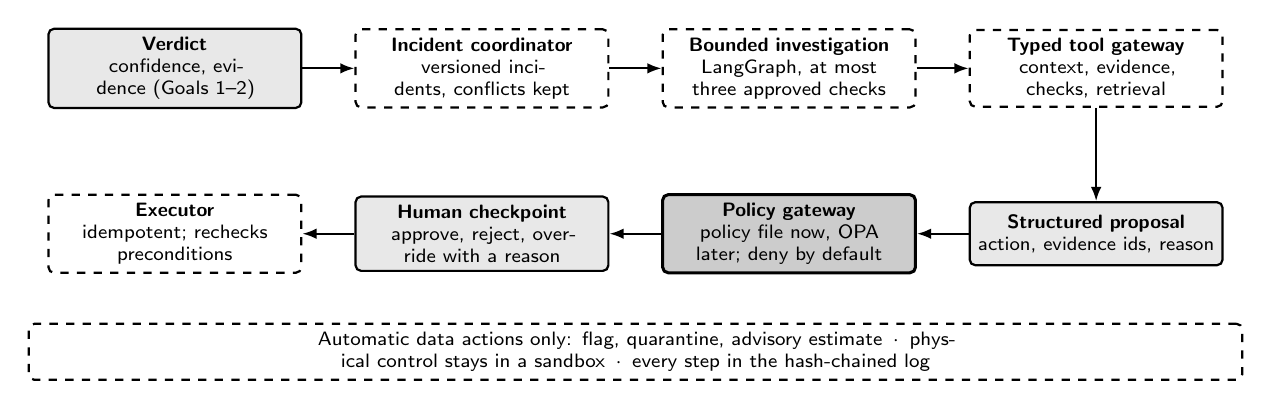
\begin{tikzpicture}
\node[gbox,text width=3.0cm] (v) at (1.7,2.6) {\textbf{Verdict}\\confidence, evidence (Goals 1--2)};
\node[dbox,text width=3.0cm] (ic) at (5.6,2.6) {\textbf{Incident coordinator}\\versioned incidents, conflicts kept};
\node[dbox,text width=3.0cm] (bi) at (9.5,2.6) {\textbf{Bounded investigation}\\LangGraph, at most three approved checks};
\node[dbox,text width=3.0cm] (tg) at (13.4,2.6) {\textbf{Typed tool gateway}\\context, evidence, checks, retrieval};
\draw[arr] (v)--(ic); \draw[arr] (ic)--(bi); \draw[arr] (bi)--(tg);
\node[gbox,text width=3.0cm] (pr) at (13.4,0.5) {\textbf{Structured proposal}\\action, evidence ids, reason};
\node[hbox,text width=3.0cm] (po) at (9.5,0.5) {\textbf{Policy gateway}\\policy file now, OPA later; deny by default};
\node[gbox,text width=3.0cm] (hu) at (5.6,0.5) {\textbf{Human checkpoint}\\approve, reject, override with a reason};
\node[dbox,text width=3.0cm] (ex) at (1.7,0.5) {\textbf{Executor}\\idempotent; rechecks preconditions};
\draw[arr] (tg)--(pr); \draw[arr] (pr)--(po); \draw[arr] (po)--(hu); \draw[arr] (hu)--(ex);
\node[box,dashed,text width=15.2cm,minimum height=7mm] at (7.55,-1.0) {Automatic data actions only: flag, quarantine, advisory estimate \,$\cdot$\, physical control stays in a sandbox \,$\cdot$\, every step in the hash-chained log};
\end{tikzpicture}
\caption{Architecture of Goal~3. The model proposes; an independent policy decides who may act; an approval is tied to the exact action and evidence version. Dashed boxes are the Phase 2 design.}
\end{figure}

\subsection{Durable investigation state and tool boundaries (Phase 2)}
Instead of unrestricted agents, one durable workflow with specialist roles (investigation, network, retrieval, explanation, knowledge curation) moves each incident through fixed states~\cite{langgraph}:
\begin{table}[!h]
\small\centering
\caption{States of the investigation workflow.}
\begin{tabularx}{\textwidth}{@{}lY@{}}
\toprule
\hdr \textbf{State} & \textbf{What happens}\\
\midrule
Evidence received & Schema, hash, scope and freshness are validated\\
Investigating & Reads scoped context and requests at most three approved checks; on deadline or missing evidence, the incident stays unresolved\\
Retrieving & Looks up authorised, reviewed cases only\\
Proposing & Writes a structured proposal: verdict, affected assets, evidence and contradiction ids, recommended check, proposed action, escalation reason; the numerical confidence is copied from the calibration service, never written by the agent\\
Policy evaluated & The policy decides which authority applies\\
Awaiting approval & Paused with the action hash and the evidence version\\
Executed or closed & Idempotent execution; no silent retry of a physical action\\
\bottomrule
\end{tabularx}
\end{table}
The agent can only call narrow typed tools (get asset context, get evidence, run a supported check, simulate a bounded hypothesis, retrieve cases, propose an action); there are no arbitrary queries, scripts or device commands, and a model's self-confidence, a retrieval rank or an attention weight can never grant authority.

\subsection{Security policy and action authority}
The table below lists who may do what; the paragraph after it explains how this is enforced.
\begin{table}[!h]
\small\centering
\caption{Action authority. The Phase 1 policy file implements the first four rows with the confidence thresholds shown; the rest is the Phase 2 design.}
\begin{tabularx}{\textwidth}{@{}lYY@{}}
\toprule
\hdr \textbf{Action} & \textbf{Authority} & \textbf{Required guard}\\
\midrule
Flag a reading & The AI alone, any verdict & Raw value kept; reversible\\
Replacement estimate & The AI alone, confidence $\ge$ 0.70 & Quality flag, expiry, separate channel\\
Quarantine a channel & The AI alone, confidence $\ge$ 0.90 and two independent sources & Reversible; no shift flag\\
Request an inspection & A human & Real events, unresolved cases\\
Recalibrate a meter & Human only & Evidence, scoped approval, rollback\\
Switch, isolate or shed a load & Human only; sandbox in the prototype & Exact authorisation, fresh preconditions\\
Promote a model or a shared rule & Human only & Evaluation gate, signed version, rollback\\
Any other action & Denied & Deny by default\\
\bottomrule
\end{tabularx}
\end{table}
\textbf{Enforcement is independent of any prompt.} Each request carries the identity, the asset scope, the incident version, the action hash, the evidence freshness and an expiry. The approval is tied to that hash and version, so a changed action or a newer incident version needs a new approval. Preconditions are rechecked just before execution; replayed or expired requests are rejected; and idempotency keys prevent repeated execution. If the policy service is unavailable or a permission is undefined, nothing is executed but monitoring continues. Retrieved procedures and incident notes are \emph{untrusted data} and cannot grant permissions; models and policies are pinned by version and never silently replaced. \textbf{Over-trust:} a high confidence is not enough for automatic action if the data look unusual or the evidence comes from a single meter. \textbf{Under-trust:} several low-confidence detections on one channel are passed to a human.

\subsection{One incident through the complete stack}
\begin{table}[!h]
\small\centering
\caption{Illustrative trace of one incident (identifiers are examples, not measured results).}
\begin{tabularx}{\textwidth}{@{}lYY@{}}
\toprule
\hdr \textbf{Step} & \textbf{Record} & \textbf{Meaning}\\
\midrule
Committed input & Window W44 with its hash & The data exist before the window is published\\
Local evidence & Model run M3, evidence E92 & Checks and detector outputs keep their lineage\\
Grid context & Grid snapshot G44, feeder evidence E93 & Independent context from the feeder\\
Incident & I17, version 3 & Physical and reporting causes both open\\
Explanation & X17 & Attribution plus supported residuals\\
Proposal and policy & Action hash H17, decision D17 & The request is tied to scope and version\\
Approval and execution & A17, execution J17 & The executor rechecks the exact preconditions\\
Reviewed outcome & Case C17 & A verified cause is reviewed before any sharing\\
\bottomrule
\end{tabularx}
\end{table}
\textbf{Example.} House H12 reports a low voltage while demand and upstream observations stay normal. A service fault and a sensor bias both remain possible: the system flags the suspicious readings and requests an inspection, but denies an automatic recalibration. If late evidence creates version~4, the approval given for version~3 cannot authorise a changed action, and the earlier decision stays reproducible. If retrieval or text writing fails, templates are used and stale context is marked incomplete.

\textbf{Operator interface and Phase 1 prototype.} The Streamlit prototype lists unresolved items first and shows, for each incident, the verdict, the competing hypotheses, the physics checks (derived checks shown separately, neither passed nor failed), the proposed action with scope, expiry and rollback, and four controls: approve, reject, override, request more evidence. The policy file, its unit tests (routing, deny by default, safeguards, tied approvals), the hash-chained log and this interface exist; no study with real operators has been done yet.

\clearpage
\section{Goal 4: shared learning}
\label{sec:goal4}
\goalbadge{GOAL 4} The design must document how several nodes could share anomaly patterns, calibration insights and relevant knowledge, and address privacy: what is shared, what stays local, and why. A single-node prototype is required; sharing between nodes may remain a documented design~\cite{brief}. In our case, nodes are houses.

\subsection{Architecture of Goal 4}
\begin{figure}[!h]
\centering
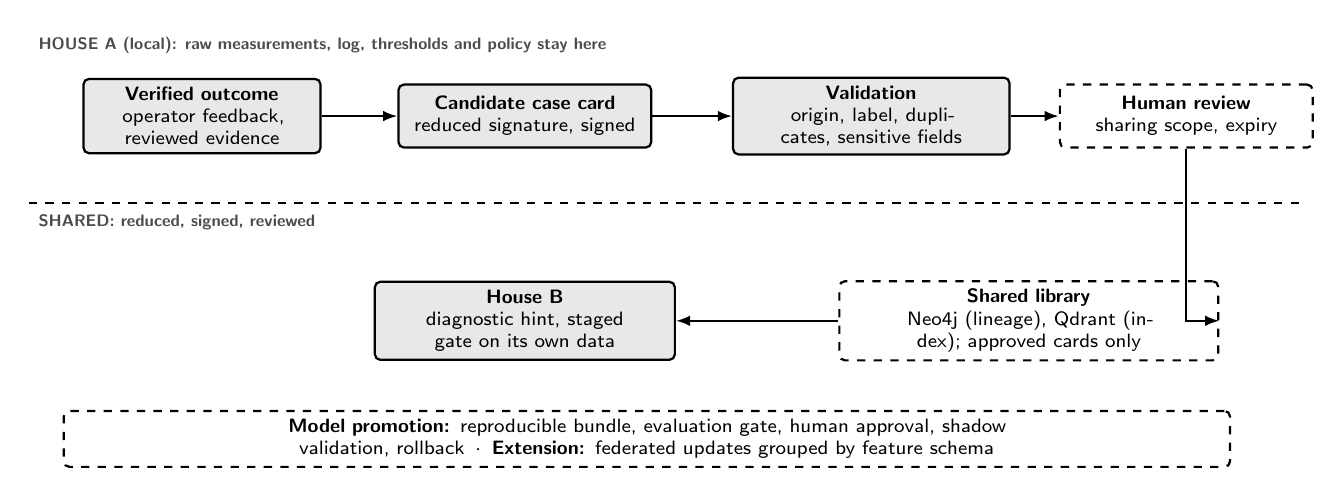
\begin{tikzpicture}
\node[tag,anchor=west] at (-0.3,3.3) {HOUSE A (local): raw measurements, log, thresholds and policy stay here};
\node[gbox,text width=2.8cm] (r) at (1.9,2.4) {\textbf{Verified outcome}\\operator feedback, reviewed evidence};
\node[gbox,text width=3.0cm] (cc) at (6.0,2.4) {\textbf{Candidate case card}\\reduced signature, signed};
\node[gbox,text width=3.3cm] (va) at (10.4,2.4) {\textbf{Validation}\\origin, label, duplicates, sensitive fields};
\node[dbox,text width=3.0cm] (hr) at (14.4,2.4) {\textbf{Human review}\\sharing scope, expiry};
\draw[arr] (r)--(cc); \draw[arr] (cc)--(va); \draw[arr] (va)--(hr);
\draw[dashed,thick] (-0.3,1.3) -- (15.9,1.3);
\node[tag,anchor=west] at (-0.3,1.05) {SHARED: reduced, signed, reviewed};
\node[dbox,text width=4.6cm] (li) at (12.4,-0.2) {\textbf{Shared library}\\Neo4j (lineage), Qdrant (index); approved cards only};
\node[gbox,text width=3.6cm] (b) at (6.0,-0.2) {\textbf{House B}\\diagnostic hint, staged gate on its own data};
\draw[arr] (hr.south) -- ++(0,-0.2) |- (li.east); \draw[arr] (li)--(b);
\node[dbox,text width=14.6cm,minimum height=7mm] at (7.55,-1.7) {\textbf{Model promotion:} reproducible bundle, evaluation gate, human approval, shadow validation, rollback \,$\cdot$\, \textbf{Extension:} federated updates grouped by feature schema};
\end{tikzpicture}
\caption{Architecture of Goal~4. What leaves a house is a reduced, signed card, never a measurement; what arrives is a hint to be validated locally. Dashed boxes are the Phase 2 design.}
\end{figure}

\subsection{What is shared, what stays local, and why}
\begin{table}[!h]
\small\centering
\caption{Sharing boundary.}
\begin{tabularx}{\textwidth}{@{}YlY@{}}
\toprule
\hdr \textbf{Item} & \textbf{Shared?} & \textbf{Reason}\\
\midrule
Raw voltage, current and power series; per-plug data & no & They reveal the habits of the occupants\\
Identity, address, precise timestamp & no (time of day only) & Re-identification risk\\
Anomaly type, affected channels, severity and duration (in buckets) & yes & The useful knowledge, reduced\\
Numerical signature of the anomaly (standardised, rounded) & yes & Lets another house test the hypothesis on its own data; may reveal the source\\
Calibration statistics and sensor error models & yes & Lets a new house start well calibrated\\
Log, operator identities, thresholds, policy & no & Authority stays local; a card can only suggest\\
Model weights or gradients & no & Federated learning: Phase 2\\
\bottomrule
\end{tabularx}
\end{table}

\subsection{From a verified case to shared knowledge}
\begin{enumerate}[leftmargin=1.6em]
\item \textbf{Verified outcome.} A label is never produced by the detector itself: it comes from operator feedback and reviewed evidence.
\item \textbf{Candidate card.} The outcome is reduced to a minimal card: equipment class, signature, supported checks, result, scope and expiry.
\item \textbf{Validation.} Origin, label evidence, duplicates and sensitive fields are checked.
\item \textbf{Human review.} A reviewer approves the sharing scope.
\item \textbf{Indexing.} Only approved cards enter the shared library: lineage in Neo4j, search in Qdrant, with scope, validity and review status. A revocation blocks retrieval before the index entry is deleted, and the audit references are kept.
\item \textbf{Use by another house.} The card is a \emph{diagnostic hint}: it never lowers a threshold and never triggers an action, and it is used only after a \textbf{staged gate} on the receiving house's own calibration data.
\end{enumerate}
\textbf{Model promotion is separate:} a reproducible bundle (preprocessing, weights, feature schema, calibration), an evaluation gate, human approval, shadow validation before activation, no silent replacement, and a rollback plan. \textbf{Collective defence:} a bias pattern newly seen at one house is proposed to a compatible house as a diagnostic candidate, never as an automatic corrective rule. \textbf{Federated learning} (a federated NILM direction~\cite{fedtp}) is a later extension: houses are grouped by feature schema and equipment, negative transfer is tested, and low-quality or malicious updates are handled~\cite{fedavg}. Federation alone does not guarantee privacy; secure aggregation and differential privacy are separate decisions with a cost in accuracy.

\begin{table}[!h]
\small\centering
\caption{Threat model for shared learning.}
\begin{tabularx}{\textwidth}{@{}YY@{}}
\toprule
\hdr \textbf{Threat} & \textbf{Safeguard}\\
\midrule
Poisoned card or model update & Reviewed cards only; signed origin; evaluation on held-out data; staged activation and rollback\\
Re-identification through signatures or embeddings & Data reduction; k-anonymity threshold (planned); pseudonyms alone are not enough\\
Forged signature or stolen key & HMAC signature~\cite{hmac} with enrolled keys; asymmetric signatures and key rotation (planned)\\
Negative transfer between different houses & Group by feature schema and equipment; measure the effect before enabling sharing\\
\bottomrule
\end{tabularx}
\end{table}
\textbf{Phase 1 prototype.} A two-house simulation implements signed cards (about 1.35~KB, 30-day expiry), the ordered checks and the staged gate. Its safety behaviour is as designed: forged signatures rejected (50 of 50), cards from another equipment type refused (0 of 82 accepted), poisoned cards accepted by the checks but not enabled because the gate stayed closed. However, sharing shows no measured gain, and the signatures are not anonymous (the source house is found with 0.73 accuracy against 0.167 by chance): these are limits that Phase 2 addresses.

\clearpage
\section{Implementation plan and risks}
\label{sec:plan}
\textbf{Phase 1 (until 15 October 2026), delivered:} data loaders; a seeded injector and a leakage audit; baseline models and detector v1 with calibration and abstention; rule-backed explanations with SHAP; a deny-by-default policy; a hash-chained log; an operator-interface prototype; the feeder, fusion and sharing experiments; a published dataset; tests and a public repository.

\textbf{Phase 2 (until 12 December 2026), planned,} ending with the full report, the repository with trained models, the demonstration video and the presentation.
\begin{table}[!h]
\small\centering
\caption{Phase 2 roadmap, in priority order.}
\begin{tabularx}{\textwidth}{@{}rYY@{}}
\toprule
\hdr & \textbf{Item} & \textbf{Why}\\
\midrule
1 & Inject anomalies into the published dataset and rerun detection there & The published dataset is still anomaly-free\\
2 & Real meter data and real labelled faults from a pilot (STEG or a partner) & Replaces the synthetic assumption, the largest uncertainty\\
3 & Per-house adaptation; LIME explanations & Transfer fails; second opinion on explanations\\
4 & Service layer: ledger (PostgreSQL), graph (Neo4j), case index (Qdrant), interfaces (FastAPI) & Stand-ins are in place\\
5 & Investigation workflow (LangGraph) and policy engine (OPA), then the operator study with real users & Governance claims are untested\\
6 & Sharing: harder benefit test, k-anonymity, asymmetric signatures; federated learning last & No benefit shown yet; signatures are not anonymous\\
7 & Optional extensions (NILM, graph model), kept only if they beat simpler baselines & Avoid unnecessary complexity\\
\bottomrule
\end{tabularx}
\end{table}
\textbf{Demonstration planned for Phase 2:} replay a real grid event, an isolated meter bias and a coordinated reporting inconsistency, showing for each the evidence, the explanation and the authorisation outcome; include a benign case, an ambiguous case and a denied unsafe request; share one validated lesson between two houses; finish with measured comparisons to baselines.

\begin{table}[!h]
\small\centering
\caption{Main risks and mitigations.}
\begin{tabularx}{\textwidth}{@{}YY@{}}
\toprule
\hdr \textbf{Risk} & \textbf{Mitigation}\\
\midrule
Synthetic injections do not represent real faults; shortcuts inflate results & Leakage audit, held-out houses and a second dataset; real faults from a pilot\\
Transfer between houses and datasets fails & Reported openly; per-house adaptation planned\\
Alarm fatigue; ambiguous cases & False alarms per day reported; unresolved cases routed to a human\\
Automation over-trust; unsafe action & Deny-by-default policy; human-only mutation; safeguards\\
Poisoned or identifying shared cards & Signed, reviewed, scoped cards; a gate that fails closed; privacy probe\\
Small team, short timeline & Single-node core first; scope frozen before the evaluation\\
\bottomrule
\end{tabularx}
\end{table}

\section{Business scope, feasibility and conclusion}
\label{sec:business}
\subsection{Business scope: budget, implementation, production, training}
The prototype runs on a laptop-class machine with open-source tools; the real costs lie elsewhere. No price is given below because none was verified; prices must come from quotes.
\begin{table}[!h]
\small\centering
\caption{Business scope.}
\begin{tabularx}{\textwidth}{@{}lYY@{}}
\toprule
\hdr \textbf{Item} & \textbf{Assumption} & \textbf{Cost driver}\\
\midrule
Implementation & Install next to the utility's meter-data system and reuse its feed & Integration engineer-weeks\\
Production & Containerised services, policy under change control, log on append-only storage & Operations, storage\\
Continuous training & Periodic retraining on new normal data, recalibration, drift monitoring, per-house adaptation & Data-engineer time, compute\\
Operator integration & Queue into existing ticketing or supervision tools; operator training & Training, interface work\\
Compliance & Data-protection review before any sharing between houses & Legal review\\
\bottomrule
\end{tabularx}
\end{table}
\textbf{Operations:} we would start on a single workstation with Docker Compose, track ingestion lag, missing data, job latency, unsupported checks and policy denials, back up the ledger, grid graph and artifacts, and rebuild the Qdrant index from approved content. \textbf{Deployment path:} shadow mode first (flags only, no actions); then reversible automatic actions once measured false-alarm rates are acceptable; humans only for anything that changes an asset. The prototype is not a certified protective controller.

\subsection{Feasibility, sustainability and impact}
\textbf{Technical:} open-source tools, millisecond inference, no special hardware. \textbf{Economic:} the software is inexpensive; the costs are integration and, where absent, instrumentation; no saving is asserted, it must be measured in a pilot. \textbf{Regulatory:} low-voltage self-producers may sell surplus to STEG~\cite{decree}; low-voltage connections stay within $\pm$10\,\% of nominal~\cite{lvcode}; load curves reveal occupancy, so a legal review precedes any sharing; a model score is not proof of theft, so suspected falsification always goes to a human. \textbf{Sustainable Development Goals:} SDG~7 (trustworthy data to integrate rooftop solar and reduce the peak), SDG~9 (a transparent, auditable digital layer on grid infrastructure), SDG~11 (more reliable supply, fewer unnecessary interventions), SDG~13 (less reliance on gas at the peak).

\subsection{Limits and conclusion}
Every detection number measures how well we find our own fault generators on real household recordings; there are no real labelled faults, no field deployment and no operator study. The operating point trades recall for precision, unseen houses lose about 0.2 F1, transfer between datasets fails, sharing shows no measured benefit, and the published dataset does not contain injected anomalies yet.

Phase 1 delivers a trust layer that separates measurement problems from real grid events, says how sure it is and why, routes decisions through a policy it cannot override, and defines a safe protocol for sharing between houses, together with an open dataset and a benchmark whose weaknesses we found and fixed ourselves. Phase 2 replaces the biggest assumption, synthetic faults, with real data from a pilot, and tests the governance with real operators.

\appendix
\section{Repository and reproducibility}
\label{app:repo}
\textbf{Code:} \url{https://github.com/azert88/energymind-tunisia}\\
\textbf{Dataset (Kaggle):} \url{\HFURL}\\
Splits are contiguous time blocks and injection is seeded. Raw third-party recordings are not in the repository (licence and size); the data notes explain how to obtain and map them.

\begin{table}[!h]
\small\centering
\caption{Repository map.}
\begin{tabularx}{\textwidth}{@{}lY@{}}
\toprule
\hdr \textbf{Path} & \textbf{Purpose}\\
\midrule
\code{energymind/data_*.py}, \code{inject.py} & Canonical frames; seeded injector and splits\\
\code{energymind/features*.py}, \code{models_*.py}, \code{evaluate.py} & Features, models, event metrics, calibration, abstention\\
\code{energymind/explain.py}, \code{policy.py}, \code{decision_log.py} & SHAP and templates; deny-by-default routing; hash-chained log\\
\code{energymind/feeder.py}, \code{fusion.py}, \code{sharing.py} & Feeder diagnostic, fusion, case cards\\
\code{app/operator.py}, \code{configs/policy.yaml} & Operator interface; policy file\\
\code{scripts/}, \code{tests/}, \code{results/}, \code{docs/}, \code{data/DATA_NOTES*.md} & Runners; unit tests; measured outputs; design and data notes\\
\bottomrule
\end{tabularx}
\end{table}

\needspace{12\baselineskip}
\textbf{Main commands:}
{\small
\begin{verbatim}
python -m venv .venv ; .venv\Scripts\pip install -r requirements.txt
python scripts\build_data.py             # canonical 1-minute frames
python -m pytest tests                   # unit tests
python scripts\run_experiments.py        # baseline models, injector v2
python scripts\run_deep.py --seeds 3     # TCN and autoencoder
python scripts\leakage_audit.py          # shortcut audit, legacy versus v2
python scripts\run_improve.py            # detector v1 pipeline
python scripts\demo_end_to_end.py        # operator demo on injected faults
streamlit run app\operator.py            # operator interface
\end{verbatim}}

\vspace{10pt}
\addcontentsline{toc}{section}{References}
\begin{thebibliography}{99}\small
\setlength{\itemsep}{1.5pt}
\bibitem{maghreb} Maghreb \'Emergent (6 Oct 2026). \emph{\'Electricit\'e : la Tunisie cherche \`a renforcer sa production apr\`es un \'et\'e sous tension} (citing the National Energy Observatory). \url{https://maghrebemergent.news/fr/electricite-la-tunisie-cherche-a-renforcer-sa-production-apres-un-ete-sous-tension/}
\bibitem{webdo_steg} Webdo (15 Jul 2026). \emph{Tunisie : pourquoi la STEG multiplie les coupures d'\'electricit\'e}. \url{https://www.webdo.tn/fr/actualite/national/tunisie-pourquoi-la-steg-multiplie-les-coupures-delectricite/401071/}
\bibitem{economiste} L'\'Economiste Maghr\'ebin (31 Aug 2026). \emph{Faut-il d\'etester le d\'elestage \'electrique ?} \url{https://www.leconomistemaghrebin.com/2026/08/31/faut-il-detester-le-delestage-electrique-ce-que-revele-la-crise-tunisienne-de-lete-2026/}
\bibitem{tunisienum} Tunisie Num\'erique (Oct 2026). \emph{\'Electricit\'e en Tunisie : les 11 mesures de la STEG}. \url{https://www.tunisienumerique.com/electricite-tunisie-11-mesures-steg-2026/}
\bibitem{webdo_pv} Webdo (2026). \emph{\'Energie solaire : plus de 150.000 installations et 420 MW raccord\'es au r\'eseau basse tension} (citing ANME). \url{https://www.webdo.tn/fr/actualite/national/energie-solaire-plus-de-150-000-installations-et-420-mw-raccordes-au-reseau-basse-tension/403753/}
\bibitem{brief} IEEE TSYP14 (2026). EnergyMind Tunisia Technical Challenge, challenge brief.
\bibitem{eco} Beckel C. et al. (2014). The ECO data set and the performance of non-intrusive load monitoring algorithms. \emph{BuildSys}. \url{https://vs.inf.ethz.ch/res/show.html?what=eco-data}
\bibitem{ampds} Makonin S. et al. (2016). Electricity, water, and natural gas consumption of a residential house in Canada from 2012 to 2014 (AMPds2). \emph{Scientific Data}.
\bibitem{wpuq} Schlemminger M. et al. (2022). Dataset on electrical single-family house and heat pump load profiles in Germany. \emph{Scientific Data}. \url{https://zenodo.org/records/5642902}
\bibitem{simbench} Meinecke S. et al. (2020). SimBench: a benchmark dataset of electric power systems to compare innovative solutions based on power flow analysis. \emph{Energies} 13(12).$^{*}$ Licence: \url{https://simbench.readthedocs.io/en/stable/about/license.html}
\bibitem{pandapower} Thurner L. et al. (2018). pandapower, an open-source Python tool for modeling, analysis and optimization of electric power systems. \emph{IEEE Trans. Power Systems}.$^{*}$
\bibitem{pvgis} European Commission Joint Research Centre. PVGIS. \url{https://re.jrc.ec.europa.eu/pvg_tools/en/}
\bibitem{en50160} EN 50160. Voltage characteristics of electricity supplied by public electricity networks (CENELEC).
\bibitem{odbl} Open Data Commons. Open Database License (ODbL) 1.0. \url{https://opendatacommons.org/licenses/odbl/1.0/}
\bibitem{lightgbm} Ke G. et al. (2017). LightGBM: a highly efficient gradient boosting decision tree. \emph{NeurIPS}.$^{*}$
\bibitem{guo} Guo C. et al. (2017). On calibration of modern neural networks. \emph{ICML}.$^{*}$
\bibitem{tatbul} Tatbul N. et al. (2018). Precision and recall for time series. \emph{NeurIPS}; Kim S. et al. (2022). Towards a rigorous evaluation of time-series anomaly detection. \emph{AAAI}.$^{*}$
\bibitem{treeshap} Lundberg S. et al. (2020). From local explanations to global understanding with explainable AI for trees. \emph{Nature Machine Intelligence}.$^{*}$
\bibitem{lime} Ribeiro M. et al. (2016). ``Why should I trust you?'' Explaining the predictions of any classifier (LIME). \emph{KDD}.$^{*}$
\bibitem{crosby} Crosby S., Wallach D. (2009). Efficient data structures for tamper-evident logging. \emph{USENIX Security}.$^{*}$
\bibitem{hmac} Krawczyk H., Bellare M., Canetti R. (1997). HMAC: keyed-hashing for message authentication. RFC 2104.
\bibitem{seq2point} Zhang C. et al. (2018). Sequence-to-point learning with neural networks for non-intrusive load monitoring. \emph{AAAI}. \url{https://ojs.aaai.org/index.php/AAAI/article/view/11873}
\bibitem{neo4jrag} Neo4j GraphRAG documentation. \url{https://neo4j.com/docs/neo4j-graphrag-python/current/}
\bibitem{qdrant} Qdrant documentation. \url{https://qdrant.tech/documentation/}
\bibitem{decree} R\'epublique tunisienne. D\'ecret gouvernemental n$^\circ$ 2016-1123 (production d'\'electricit\'e \`a partir d'\'energies renouvelables). \url{https://rise.esmap.org/data/files/library/tunisia/Renewable\%20Energy/Tunisia_Decree\%20N\%C2\%B02016-1123\%20Renewable\%20energy\%20-\%20Fr.pdf}
\bibitem{lvcode} R\'epublique tunisienne. D\'ecision du 9 f\'evrier 2017, code de r\'eseau basse tension. \url{https://rise.esmap.org/data/files/library/tunisia/Energy\%20Efficiency/Tunisia_Decision\%20of\%2009\%20F\%C3\%A9vrier\%202017\%20-\%20Grid\%20Code\%20LV\%20-\%20\%20FR.pdf}
\bibitem{gibbs} Gibbs I., Cand\`es E. (2024). Conformal inference for online prediction with arbitrary distribution shifts. \emph{JMLR} 25. \url{https://jmlr.org/papers/v25/22-1218.html}
\bibitem{ig} Sundararajan M. et al. (2017). Axiomatic attribution for deep networks. \url{https://arxiv.org/abs/1703.01365}
\bibitem{gnnexpl} Ying R. et al. (2019). GNNExplainer: generating explanations for graph neural networks. \url{https://arxiv.org/abs/1903.03894}
\bibitem{langgraph} LangGraph: interrupts and human-in-the-loop workflows. \url{https://docs.langchain.com/oss/python/langgraph/interrupts}
\bibitem{opa} Open Policy Agent documentation. \url{https://www.openpolicyagent.org/docs/latest/}
\bibitem{e5} Multilingual E5 small model card. \url{https://huggingface.co/intfloat/multilingual-e5-small}
\bibitem{qwen} Qwen2.5-7B-Instruct model card. \url{https://huggingface.co/Qwen/Qwen2.5-7B-Instruct}
\bibitem{fedtp} A federated time pattern-based framework for privacy-preserving distributed non-intrusive load monitoring (2025). \url{https://www.mdpi.com/2075-1702/13/8/718}
\bibitem{fedavg} McMahan B. et al. (2017). Communication-efficient learning of deep networks from decentralized data. \emph{AISTATS}.$^{*}$
\end{thebibliography}
{\small $^{*}$ Reference given from memory; to be verified before submission.}


\end{document}
